%% State Space Modelling of Dynamic Systems
%% Lecture 1: Introduction to State-Space Models
\def\FileDate{9/9/29}
\def\FileVersion{1.1}
% ----------------------------------------------------------------
% Notes pages *********************************************************
% ----------------------------------------------------------------
The state-space model is a form of system representation that is used
in several engineering disciplines. It is particularly used in control
and in signal processing.

The state-space model is a form of differential equation
representation and it is principally used when an analysis of the
system behaviour is required in terms of time responses. That
stated, it is relatively easy to convert a state-space model into
a transfer function, to allow the frequency response analysis of a
system. It is however not necessary to do this conversion if the
time-response behaviour is all that is required.

The state space model is easily extended to cope with models with more
than one input and more than one output. It also has more favourable
numerical properties that make it more attractive as a representation
for high order systems\footnote{Systems with large numbers of
  derivative terms} than the polynomial representation provided by the
transfer function. State-space models are easily simulated by the
straightforward application of numerical integration.

\sref{slide:l1s1} shows a simple electrical circuit. We shall develop
this circuit into a block diagram and from the block-diagram we shall
develop the state-space model.

\begin{slide}\label{slide:l1s1}
\heading{Example}
\begin{center}
\resizebox{150pt}{!}{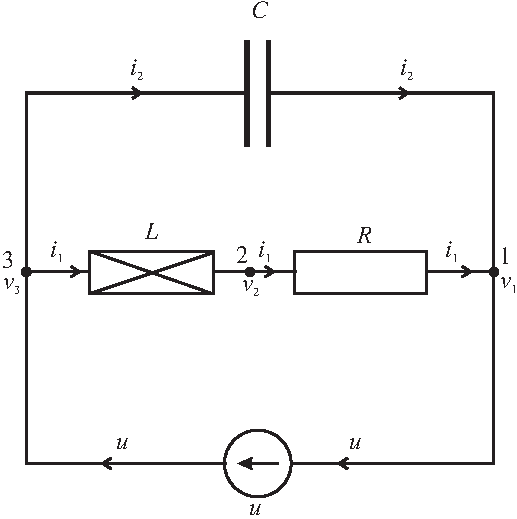
\includegraphics{pictures/circuit.pdf}}
\end{center}
\end{slide}


\ifslidesonly
\begin{slide}\label{opteq:l1e1a}
\heading{Equations}
If we write down the equations for the elements we get:
\begin{eqnarray*}
  \frac{dv_{31}}{dt} &=& \frac{1}{C}\ i_2 \\
  \frac{di_{i}}{dt} &=& \frac{1}{L}\ v_{32} \\
  v_{21} &=& R\ i_1
\end{eqnarray*}
The ``compatability'' and ``continuity'' equations are
\begin{eqnarray*}
  u &=& i_1 + i_2 \\
  v_{31} &=& v_{32} + v_{21}
\end{eqnarray*}

\endinput
%%% Local Variables: 
%%% mode: latex
%%% TeX-master: "notes"
%%% End: 

\end{slide}
\fiIf we write down the equations for the elements we get:
\begin{eqnarray*}
  \frac{dv_{31}}{dt} &=& \frac{1}{C}\ i_2 \\
  \frac{di_{i}}{dt} &=& \frac{1}{L}\ v_{32} \\
  v_{21} &=& R\ i_1
\end{eqnarray*}
The ``compatability'' and ``continuity'' equations are
\begin{eqnarray*}
  u &=& i_1 + i_2 \\
  v_{31} &=& v_{32} + v_{21}
\end{eqnarray*}

\endinput
%%% Local Variables: 
%%% mode: latex
%%% TeX-master: "notes"
%%% End: 



Since the system ``source'' is $u$, we can construct the block diagram
systematically by tracing the equations through from the source. We
also introduce the additional constraint that we would like the derivative terms
$dv_{31}/dt$ and $di_1/dt$ to
appear as inputs to integrator blocks whose outputs are therefore
\ifslidesonly
\begin{slide}\label{opteq:l1e1b}
\heading{Equations (continued)}
Integrator equations:
\begin{eqnarray*}
  v_{31} = \int \frac{dv_{31}}{dt} dt \\
  i_{1} = \int \frac{i_{1}}{dt} dt
\end{eqnarray*}

\endinput
%%% Local Variables: 
%%% mode: latex
%%% TeX-master: "notes"
%%% End: 

\end{slide}
\fi\begin{eqnarray*}
  v_{31} = \int \frac{dv_{31}}{dt} dt \\
  i_{1} = \int \frac{i_{1}}{dt} dt
\end{eqnarray*}

\endinput
%%% Local Variables: 
%%% mode: latex
%%% TeX-master: "notes"
%%% End: 

The other
components of equations (\ref{eq:l1e1}) to (\ref{eq:l1e3}) appear as
gain blocks and (\ref{eq:l1e4}) and (\ref{eq:l1e5}) appear as summing
junctions.  With these constraints, the resulting block diagram is
that shown in \sref{slide:l1s2}.

We can model these equations in \Matlab{}/\Simulink{}\footnote{Note
  that in \Simulink{} triangular blocks are used for gains and that the transfer function
  block $1/s$ represents the integral operator $\int$. The small
  elliptical blocks represent input and output ports.} as shown in \sref{slide:l1s1a}.
\begin{slide}\label{slide:l1s1a}
\heading{Modelled Equations}
\resizebox{300pt}{!}{\rotatebox{90}{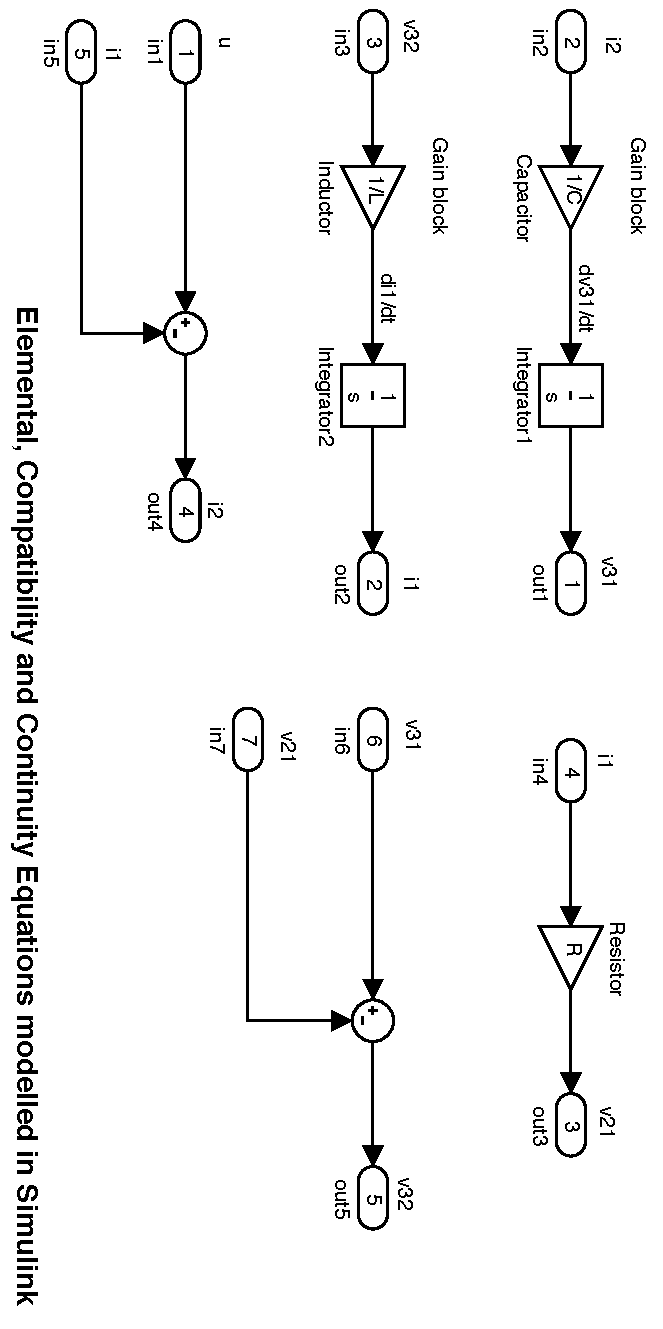
\includegraphics{pictures/blocks.pdf}}}
\end{slide}
Combining these blocks such that the input is $u$ and the output is
the current flowing through the inductance $i_1$\footnote{We could have used any signal as an output as we shall
  see later.} we obtain the block diagram shown in \sref{slide:l1s2}.
\begin{slide}\label{slide:l1s2}
\heading{Example as a Block Diagram}
\resizebox{300pt}{!}{\rotatebox{90}{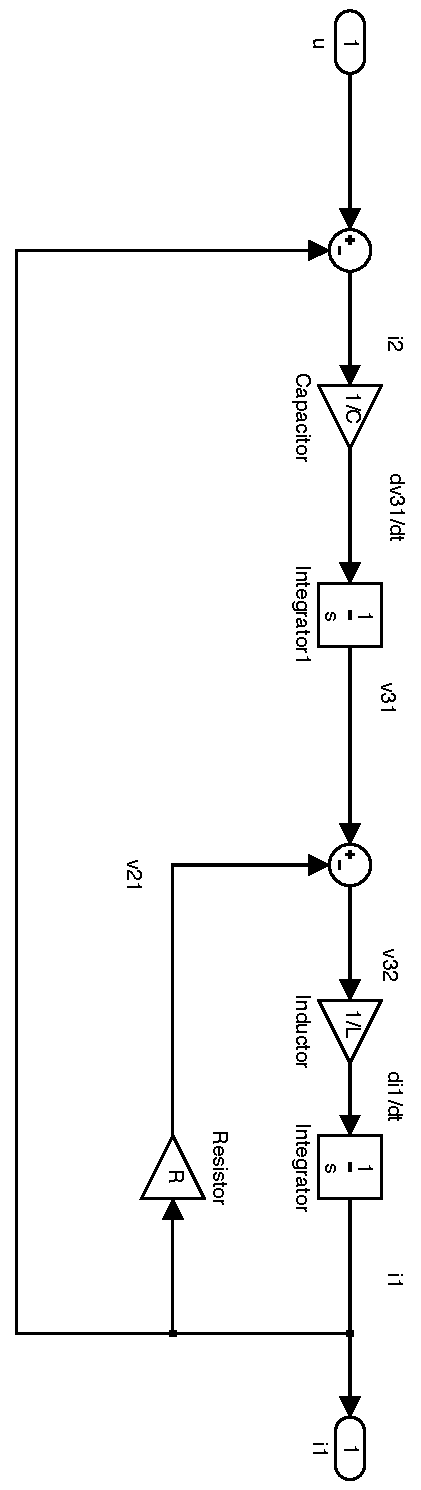
\includegraphics{pictures/blockdiag.pdf}}}
\end{slide}

Having constructed a block diagram that allows us the visualize
the structure of the differential equations, we now go on to
create the state-space model of the system. To do this we first
identify the ``\emph{state-variables}'' which are (in this case)
the physical quantities that are changing with time, i.e. the
voltage across the capacitor $v_{31}$ and the current through the
inductor $i_1$\footnote{A state variable that can be related to a
physical quantity is called a ``\emph{physical state
variable}.''}. The derivatives of these state variables become the
left-hand-side of the ``\emph{state equations}''. These equations
have apparently already been written down as (\ref{eq:l1e1}) and
(\ref{eq:l1e2}), but we impose an additional condition that the
state equations can only involve the state-variables, their
derivatives and the system input. Thus we have to trace the path
back through the block diagram from the inputs to the integrator
blocks to the (nearest) state variable(s). The result is
\ifslidesonly
shown in \sref{slide:ss1}
\begin{slide}\label{slide:ss1}
\heading{State Equations for the Example}
For example, if\ifnotes\footnote{$\epsilon(t)$ is the unit step function
  $\epsilon(t)=0$ for $t < 0$; $\epsilon(t)=1$ for $t \ge 0$.}\fi
\begin{displaymath}
  \mathbf{v}(t)=\left[ \begin{array}{c}
   \epsilon(t) \\
   e^{-at} \\
   \sin bt \\
  \end{array} \right]
\end{displaymath}
then
\begin{displaymath}
  \mathbf{V}(s)=\left[ \begin{array}{c}
   1/s \\
   1/s+a \\
   b/(s^2+b^2) \\
  \end{array} \right]
\end{displaymath}

\endinput

%%% Local Variables: 
%%% mode: latex
%%% TeX-master: "notes"
%%% End: 

\end{slide}
\fiFor example, if\ifnotes\footnote{$\epsilon(t)$ is the unit step function
  $\epsilon(t)=0$ for $t < 0$; $\epsilon(t)=1$ for $t \ge 0$.}\fi
\begin{displaymath}
  \mathbf{v}(t)=\left[ \begin{array}{c}
   \epsilon(t) \\
   e^{-at} \\
   \sin bt \\
  \end{array} \right]
\end{displaymath}
then
\begin{displaymath}
  \mathbf{V}(s)=\left[ \begin{array}{c}
   1/s \\
   1/s+a \\
   b/(s^2+b^2) \\
  \end{array} \right]
\end{displaymath}

\endinput

%%% Local Variables: 
%%% mode: latex
%%% TeX-master: "notes"
%%% End: 


Equations (\ref{eq:l1e6}) and (\ref{eq:l1e7}) together form a pair
of simultaneous equations (they must both be satisfied by the
dynamic response of the circuit voltages and currents to the
input) and they may therefore be written in vector
form\footnote{You should expand this matrix equation
(\ref{eq:l1e8}) out to verify that it is equivalent to
(\ref{eq:l1e6}) and (\ref{eq:l1e7}).}:
\begin{equation}\label{eq:l1e8}
  \left[\begin{array}{c}
    dv_{31}/dt \\
    di_{i}/dt \\
    \end{array}\right]=\left[\begin{array}{cc}
      0 & -1/C \\
      1/L & -R/L \\
    \end{array}\right]\left[\begin{array}{c}
      v_{31} \\
      i_1 \\
    \end{array}\right]+\left[\begin{array}{c}
      1/C \\
      0 \\
    \end{array}\right]\ u
\endinput
%%% Local Variables: 
%%% mode: latex
%%% TeX-master: "notes"
%%% End: 

\end{equation}
\ifslidesonly
\begin{slide}
\heading{State equations in vector form}
\begin{displaymath}
  \left[\begin{array}{c}
    dv_{31}/dt \\
    di_{i}/dt \\
    \end{array}\right]=\left[\begin{array}{cc}
      0 & -1/C \\
      1/L & -R/L \\
    \end{array}\right]\left[\begin{array}{c}
      v_{31} \\
      i_1 \\
    \end{array}\right]+\left[\begin{array}{c}
      1/C \\
      0 \\
    \end{array}\right]\ u
\endinput
%%% Local Variables: 
%%% mode: latex
%%% TeX-master: "notes"
%%% End: 

\end{displaymath}
The transform equations may be solved as follows (the Laplace
transform operator $s$ is omitted for brevity).

\begin{eqnarray}
 s\mathbf{X}-\mathbf{x}(0) &=&
  \mathbf{A}\mathbf{X}+\mathbf{B}\mathbf{U}\nonumber\\
 s\mathbf{X}-\mathbf{A}\mathbf{X} &=&
  \mathbf{B}\mathbf{U}+\mathbf{x}(0)\nonumber\\
 \left[s\mathbf{I}-\mathbf{A}\right]\mathbf{X} &=&
  \mathbf{B}\mathbf{U}+\mathbf{x}(0)\nonumber\\
 \mathbf{X} &=&
  \left[s\mathbf{I}-\mathbf{A}\right]^{-1}\mathbf{B}\mathbf{U}+
  \left[s\mathbf{I}-\mathbf{A}\right]^{-1}\mathbf{x}(0)\label{eqn:def-of-x}\\
  \mathrm{and}\nonumber \\
  \mathbf{Y}&=& \mathbf{C}\mathbf{X}+\mathbf{D}\mathbf{U}\label{eqn:def-of-y}
\end{eqnarray}

\endinput

%%% Local Variables: 
%%% mode: latex
%%% TeX-master: "notes"
%%% End: 

\end{slide}
\fi
The transform equations may be solved as follows (the Laplace
transform operator $s$ is omitted for brevity).

\begin{eqnarray}
 s\mathbf{X}-\mathbf{x}(0) &=&
  \mathbf{A}\mathbf{X}+\mathbf{B}\mathbf{U}\nonumber\\
 s\mathbf{X}-\mathbf{A}\mathbf{X} &=&
  \mathbf{B}\mathbf{U}+\mathbf{x}(0)\nonumber\\
 \left[s\mathbf{I}-\mathbf{A}\right]\mathbf{X} &=&
  \mathbf{B}\mathbf{U}+\mathbf{x}(0)\nonumber\\
 \mathbf{X} &=&
  \left[s\mathbf{I}-\mathbf{A}\right]^{-1}\mathbf{B}\mathbf{U}+
  \left[s\mathbf{I}-\mathbf{A}\right]^{-1}\mathbf{x}(0)\label{eqn:def-of-x}\\
  \mathrm{and}\nonumber \\
  \mathbf{Y}&=& \mathbf{C}\mathbf{X}+\mathbf{D}\mathbf{U}\label{eqn:def-of-y}
\end{eqnarray}

\endinput

%%% Local Variables: 
%%% mode: latex
%%% TeX-master: "notes"
%%% End: 
\footnote{The matrix
operator $[]^T$ is the ``transpose'' operator. In this case it
converts the row vector shown into the column vector actually used
in the state equations. When applied to a matrix, the rows of the
matrix become the columns of the transposed matrix. We shall use
the transpose operator in the discussion of state equations to
avoid messy attempts to write column vectors in the body of a
sentence!}

We can generalize this result by defining general state variables
$x_1=v_{31}$ and $x_2=i_1$. Using the notational shorthand
$\dot{x}=dx/dt$ we then get:
\begin{equation}\label{eq:l1e9}
  \left[\begin{array}{c}
    \dot{x_1} \\
    \dot{x_2} \\
    \end{array}\right]=\left[\begin{array}{cc}
      0 & -1/C \\
      1/L & -R/L \\
    \end{array}\right]\left[\begin{array}{c}
      x_1 \\
      x_2 \\
    \end{array}\right]+\left[\begin{array}{c}
      1/C \\
      0 \\
    \end{array}\right]\ u
\end{equation}
\ifslidesonly
\begin{slide}
\heading{Generalising the Equations}
We can generalize the result by defining general state variables
$x_1=v_{31}$ and $x_2=i_1$. Using the notational shorthand
$\dot{x}=dx/dt$ we then get:
\begin{displaymath}
  \left[\begin{array}{c}
    \dot{x_1} \\
    \dot{x_2} \\
    \end{array}\right]=\left[\begin{array}{cc}
      0 & -1/C \\
      1/L & -R/L \\
    \end{array}\right]\left[\begin{array}{c}
      x_1 \\
      x_2 \\
    \end{array}\right]+\left[\begin{array}{c}
      1/C \\
      0 \\
    \end{array}\right]\ u
\end{displaymath}
\end{slide}
\fi
In general, we will have $n$ state variables and $q$ system
inputs. In such a case we can write down a general matrix state
equation as developed in \sref{slide:l1s3} and \sref{slide:l1s4}.
\begin{slide}\label{slide:l1s3}
\heading{General State Equation (1)} Let us define a general
$n$-dimensional state vector
\[\mathbf{x} = \left[x_1,\ x_2,\ \ldots, x_n\right]^T\] Its
derivative is
\[\frac{d\mathbf{x}}{dt} = \left[\frac{dx_1}{dt},\ \frac{dx_2}{dt},\
\ldots,\
\frac{dx_n}{dt}\right]^T\] or more compactly
\[\dot{\mathbf{x}}=\left[\dot{x_1},\ \dot{x_2},\ \ldots,\
\dot{x_n}\right]^T.\]

There may be any number of inputs to a system, so we also assume a
general vector of $q$ inputs
\[\mathbf{u}=\left[u_1,\ u_2,\ \ldots,\ u_q\right]^T\]
\end{slide}

\begin{slide}\label{slide:l1s4}
\heading{General State Equation (2)}
\[
\dot{\mathbf{x}}=\left[\begin{array}{cccc}
  a_{11} & a_{12} & \cdots & a_{1n} \\
  a_{21} & a_{22} & \cdots & a_{2n} \\
  \vdots & \vdots & \ddots & \vdots \\
  a_{n1} & a_{n2} & \cdots & a_{nn}
\end{array}\right]\ \mathbf{x} + \left[\begin{array}{cccc}
  b_{11} & b_{12} & \cdots & b_{1q} \\
  b_{21} & b_{22} & \cdots & b_{2q} \\
  \vdots & \vdots & \ddots & \vdots \\
  b_{n1} & b_{n2} & \cdots & b_{nq}
\end{array}\right]\ \mathbf{u} \\
\]
or more succinctly
\[
\dot{\mathbf{x}}=\mathbf{A}\mathbf{x}+\mathbf{B}\mathbf{u}
\]
Where $\mathbf{A}$ is the $n\times n$ ``\emph{system matrix}'' and
$\mathbf{B}$ is the $n\times q$ ``\emph{input matrix}''.
\end{slide}


The state equations allow us to describe the internal behaviour of
the system when subjected to stimuli from the inputs. In the
example, we need nothing more if we wish to describe the way that
the capacitor voltage $v_{31}$ and inductor current $i_1$ change
with time under the influence of the input current $u$. However,
if we wish to describe the behaviour of the other variables in the
circuit we need to complete the state space model with a set of
``\emph{output equations}.''

Let us consider every possible output. From the block diagram, we
see that, in terms of the state variables and the system input
\begin{eqnarray}
\label{eq:l1y1} v_{31}&=&1\times v_{31} \\
i_1 & = & 1\times i_1 \\
v_{32} &=& 1\times v_{31} - R \times i_1 \\ 
v_{21} & = & R \times i_1 \\ 
\label{eq:l1yn} i_2 & = & u - 1\times i_1.
\end{eqnarray}
\ifslidesonly
\begin{slide}
\heading{Output Equations}
For illustration purposes we write an ``output equation'' for every
possible signal.
\begin{eqnarray*}
v_{31}&=&1\times v_{31} \\
i_1 & = & 1\times i_1 \\ 
v_{32} &=& 1\times v_{31} - R \times i_1 \\ 
v_{21} & = & R \times i_1\\ 
i_2 & = & u - 1\times i_1.
\end{eqnarray*}
\end{slide}
\fi
Arranging these equations in vector form we have:
\begin{equation}
\left[\begin{array}{c}
  v_{31} \\
  i_1 \\
  v_{32} \\
  v_{21} \\
  i_2
\end{array}\right] = \left[\begin{array}{cc}
  1 & 0 \\
  0 & 1 \\
  1 & -R \\
  0 & R \\
  0 & -1
\end{array}\right]\ \left[\begin{array}{c}
  v_{31} \\
  i_1
\end{array}\right]+\left[\begin{array}{c}
  0 \\
  0 \\
  0 \\
  0 \\
  1
\end{array}\right] u
\end{equation}
\ifslidesonly
\begin{slide}
\heading{Vectorised form...}
Arranging the ouput equations in vector form we have:
\begin{displaymath}
\left[\begin{array}{c}
  v_{31} \\
  i_1 \\
  v_{32} \\
  v_{21} \\
  i_2
\end{array}\right] = \left[\begin{array}{cc}
  1 & 0 \\
  0 & 1 \\
  1 & -R \\
  0 & R \\
  0 & -1
\end{array}\right]\ \left[\begin{array}{c}
  v_{31} \\
  i_1
\end{array}\right]+\left[\begin{array}{c}
  0 \\
  0 \\
  0 \\
  0 \\
  1
\end{array}\right] u
\end{displaymath}
\end{slide}
\fi
In general, we can describe a system with $r$ inputs in terms of
the generic output variables $y_1, y_2,\ldots,\ y_r$ as shown in
\sref{slide:l1s5} and \sref{slide:l1s6}.
\begin{slide}\label{slide:l1s5}
\heading{General Output Equation (1)} Let us define a general
output vector
\[\mathbf{y} = \left[y_1,\ y_2,\ \ldots, y_r\right]^T\]

Given that some of the inputs to the system may be directly
connected to the output, the input vector may also appear in the
output general equation.
\end{slide}
\begin{slide}\label{slide:l1s6}
\heading{General Output Equation (2)}
\[
\mathbf{y}=\left[\begin{array}{cccc}
  c_{11} & c_{12} & \cdots & c_{1n} \\
  c_{21} & c_{22} & \cdots & c_{2n} \\
  \vdots & \vdots & \vdots & \vdots \\
  c_{r1} & c_{r2} & \cdots & c_{rn}
\end{array}\right]\ \mathbf{x} + \left[\begin{array}{cccc}
  d_{11} & d_{12} & \cdots & d_{1q} \\
  d_{21} & d_{22} & \cdots & d_{2q} \\
  \vdots & \vdots & \vdots & \vdots \\
  d_{r1} & d_{r2} & \cdots & d_{rq}
\end{array}\right]\ \mathbf{u} \\
\]
or more succinctly
\[
\mathbf{y}=\mathbf{C}\mathbf{x}+\mathbf{D}\mathbf{u}
\]
Where $\mathbf{C}$ is the $n\times r$ ``\emph{output matrix}'' and
$\mathbf{D}$ is the $r\times q$ ``\emph{feedforward matrix}''.
\end{slide} This
equation relates the states and inputs to the outputs. There are
no dynamic terms!
\begin{slide}\label{slide:l1s7}
\heading{The State Space Model}
\begin{eqnarray*}
\dot{\mathbf{x}}&=&\mathbf{A}\mathbf{x}+\mathbf{B}\mathbf{u}\\
{y}&=&\mathbf{C}\mathbf{x}+\mathbf{D}\mathbf{u}
\end{eqnarray*}
Can always be developed from a system with physically realizable
states and physical realistic sources. Such a system is called
``\emph{proper}''. If $\mathbf{D}$ is null (matrix of zeros) the
system is called ``\emph{strictly proper}''.
\end{slide}
A block diagram representation of the state space model is shown
in \sref{slide:l1s8}. The block diagram of the circuit, rearranged
to match the general model is shown in \sref{slide:l1s9}.
\begin{slide}\label{slide:l1s8}
\heading{Block Diagram of a State-Space Model}
\resizebox{300pt}{!}{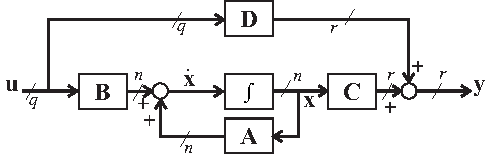
\includegraphics{pictures/ssmodel}}
\end{slide}
\begin{slide}\label{slide:l1s9}
\heading{State Space Model of the Example}
\resizebox{300pt}{!}{\rotatebox{90}{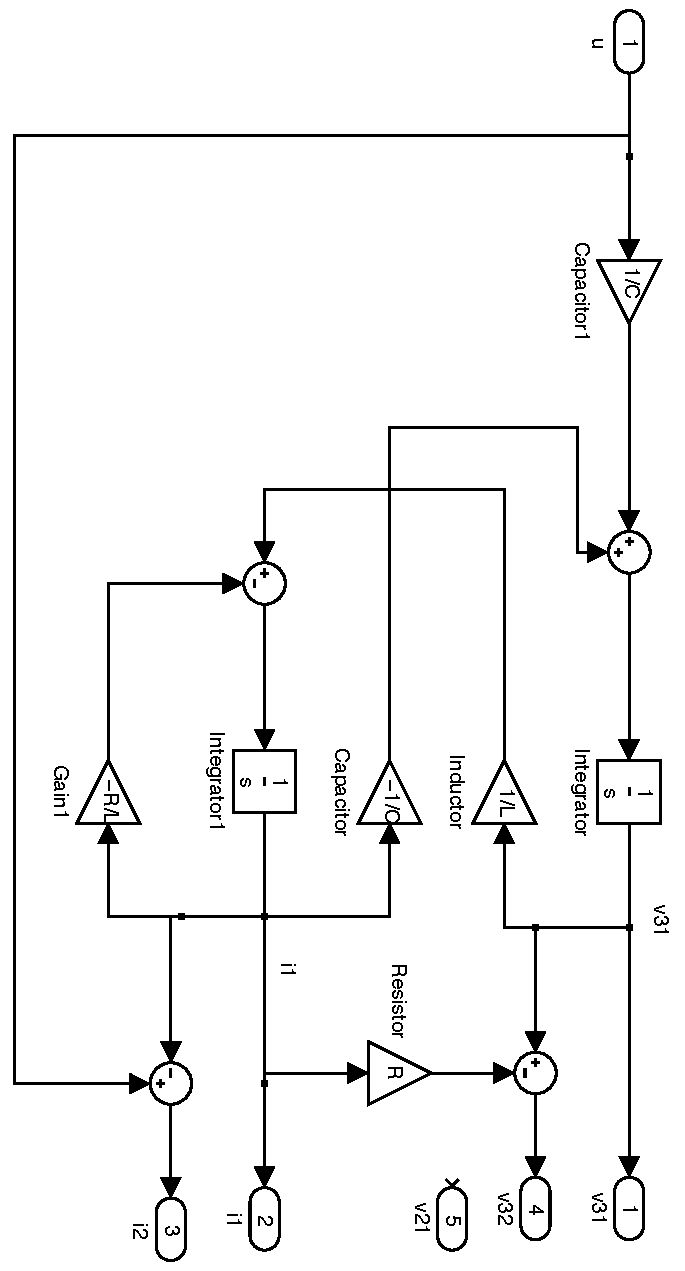
\includegraphics{pictures/statemodel.pdf}}}
\end{slide}
%----------------------------------------------------------------
% The end of slides
% ----------------------------------------------------------------
\endinput

% Local Variables:
% TeX-master: "lecture1"
% End:
